\chapter{Latent Space Analysis}
\label{chap:latent_space_analysis}

\chapterepigraph*[I am a life form that emerged from the sea of information.]
{\textjapanese{私は情報の海で発生した生命体だ}}
{Mamoru Oshii, \textit{Ghost in the Shell} (1995)~\parencite{oshii1995ghost}}

\chaptercontents

\glsresetall

In classical machine learning approaches, practitioners had to manually design data representations in order to make them usable by simple models.
\gls{dl} introduces a paradigm shift.
Rather than relying on hand-crafted features to meaningfully represent data, it automatically learns these representations.
Through the successive activation of hidden layers, \glspl{nn} gradually construct representations that become increasingly relevant to the task under consideration \parencite{rumelhart1986learning}.

These representations are not meaningful at initialization, they emerge progressively during training as the model optimizes its objective.
It is through these learned representations that a trained network is able to map an input to an output, including for examples never encountered during training.
Since these representations are learned internally by the network and are not directly observable from the input or output spaces, they are commonly referred to as \glspl{lr}.
The collection of these \glspl{lr} learned throughout the network is referred to as a \gls{ls}.

These \glspl{ls} are now at the core of a growing number of practical applications, among which:
\begin{itemize}
    \item \textbf{Video compression:} Neural video compression exploits the compactness of \glspl{ls} to encode information efficiently \parencite{lu2019dvcendtoenddeepvideo}.
    \item \textbf{Exploration in \gls{rl}:} Agent internal representations are used for efficient exploration in extremely open environments \parencite{burda2018largescalestudycuriositydrivenlearning}.
    \item \textbf{Recommendation systems:} Users and content are modeled within a shared \gls{ls} to compute meaningful similarities \parencite{he2017neuralcollaborativefiltering}.
    \item \textbf{Retrieval-augmented generation:} Knowledge bases are indexed and queried through \glspl{lr} \parencite{lewis2021retrievalaugmentedgenerationknowledgeintensivenlp}.
    \item \textbf{Multimodal models:} \Glspl{llm} and multimodal architectures rely on the quality of learned representations to align heterogeneous modalities such as text, images, and audio \parencite{radford2021learningtransferablevisualmodels}.
\end{itemize}
These examples represent only some of the most widespread applications of \glspl{lr}.

Given their extensive use, the study of \glspl{lr} has become a central topic in \gls{dl} research.
A major objective is to understand how information is organized within these spaces, which concepts are encoded, and how these \glspl{lr} influence model behavior.

The remainder of this chapter is organized as follows:
\begin{itemize}
    \item Section~\ref{sec:latent_space_analysis_concept_hypothesis} introduces the hypothesis that underlies much of the research on \gls{ls} analysis, which we refer to as the \ConceptHypothesisName.
    \item Sections~\ref{sec:latent_space_analysis_probing}, \ref{sec:latent_space_analysis_directions}, \ref{sec:latent_space_analysis_superposition}, and \ref{sec:latent_space_analysis_clustering} examine four families of \gls{ls} analysis methods, respectively based on probing, interpretable directions, feature superposition, and clustering.
    \item Section~\ref{sec:latent_space_analysis_conclusion} concludes with a comparative synthesis of these methods and a discussion of the open questions that remain.
\end{itemize}

\section{Concept Hypothesis}
\label{sec:latent_space_analysis_concept_hypothesis}

In this section, we introduce the main working hypothesis underlying much of the literature on \gls{ls} analysis.  
Although rarely stated explicitly, this hypothesis is implicitly present in the recurring use of notions such as abstraction, representation, \gls{ls}, concept, and semantics.
Throughout this thesis, we refer to this hypothesis as \ConceptHypothesisName.
The goal of this section is to make this conceptual framework explicit by defining its main components.  

The \ConceptHypothesisName originates from the need to explain the generalization ability of deep \glspl{nn} observed after training, as discussed in Section~\ref{sec:deep_learning_evaluation}.
A model is said to generalize when, for an input $\vect{x} \in \mathcal{X}$ not seen during training, it still produces an output $\hat{\vect{y}}$ close to the true output $\vect{y}$.  
Such behavior cannot be explained by simple memorization of training samples.  
Instead, the model must extract and exploit underlying regularities in the target function.  
This requires a process of abstraction, as defined in Definition~\ref{def:abstraction}, whereby raw inputs are transformed into internal structures that are meaningful for the task \parencite{bengio2014representationlearningreviewnew}.  

\begin{definition}{Abstraction}{abstraction}
Abstraction is the process by which a model transforms an input into a task-relevant internal form.  
It captures and restructures information in order to represent relationships that are useful for prediction.  
\end{definition}

The ability of \glspl{nn} to perform abstraction arises from their intermediate activations.
A \gls{nn} does not directly map $\vect{x}$ to $\hat{\vect{y}}$, it computes a sequence of intermediate activations across hidden layers.
These activations are numerical encodings of the input referred to as embeddings.
Once training is complete, these embeddings are structured to support the performance of a specific task.
To mark this distinction, we will refer to these trained embeddings as \glspl{lr}, as defined in Definition~\ref{def:representation}.

\begin{definition}{Latent Representation}{representation}
A \gls{lr} is the internal encoding of an input given by an intermediate layer of a trained \gls{nn}.
\end{definition}

Each hidden layer refines the \gls{lr} of the previous layer.
Each transformation progressively reshapes the \gls{lr} into a form more directly aligned with the output space \parencite{rumelhart1986learning}.
This process can be described as a sequence of transformations where each $\latentRepresentation[l]$ is a \gls{lr}:
\[
\vect{x} \rightarrow \latentRepresentation[1] \rightarrow \latentRepresentation[2] \rightarrow \dots \rightarrow \latentRepresentation[L-1] \rightarrow \hat{\vect{y}}.
\]

The set of all such \glspl{lr} produced by a layer over a dataset defines its \gls{ls}, as defined in Definition~\ref{def:latent_space}.

\begin{definition}{Latent Space}{latent_space}
The \gls{ls} is the set of all \glspl{lr} produced by a layer over a dataset.
It is shaped by learning and organizes \glspl{lr} according to task-relevant properties.
\end{definition}

Under the \ConceptHypothesisName, the analysis of the \gls{ls} is assumed to provide access to abstract structures learned by the model, as illustrated in Figure~\ref{fig:latent_space}.
The same set of \glspl{lr} can be viewed either as an unstructured point cloud or, under this hypothesis, as a collection of points organized by concept membership, in which case the structure of the \gls{ls} becomes meaningful and amenable to analysis.
In Figure~\ref{fig:latent_space}, the colors represent hypothetical concept memberships assigned by the model.

In this thesis, a concept is defined as an abstract representation that organizes information and supports reasoning (see Definition~\ref{def:concept}).

\providecommand{\lsePanelWidth}{6cm}

\newlength{\lsePanelWd}
\newlength{\lsePanelHt}
\newlength{\lsePanelGap}

\begin{figure}[t]
\centering

% ================================================================
%  latent_space_shared.tex
%  Couleurs, macros et styles partagés par toutes les figures
%  latent_space_*.tex
%  Usage : \input{figures/latent_space_analysis/latent_space_shared.tex}
% ================================================================

% ----------------------------------------------------------------
% Couleurs des clusters
% ----------------------------------------------------------------
\colorlet{colorA}{blue!70!cyan}
\colorlet{colorB}{orange}
\colorlet{colorC}{green!60!black}

% Couleurs de directions (latent_space_directions.tex)
\colorlet{colorDirBA}{violet}
\colorlet{colorDirBC}{red!70!black}

% ----------------------------------------------------------------
% Macros de dessin
% ----------------------------------------------------------------
\input{figures/latent_space_analysis/plot_points.tex}
\input{figures/latent_space_analysis/plot_ellipse.tex}
\input{figures/latent_space_analysis/plot_probe.tex}
\input{figures/latent_space_analysis/plot_direction.tex}

% ----------------------------------------------------------------
% Styles d'axe partagés
% ----------------------------------------------------------------
\pgfplotsset{
  % Axe standard (clustering, probing, directions)
  latent axis/.style={
    width=11cm,
    height=10cm,
    xmin=-7, xmax=8,
    ymin=-7, ymax=5.5,
    axis x line=bottom,
    axis y line=left,
    axis line style={
      -{Stealth[length=8pt, width=6pt]},
      thick
    },
    ticks=none,
    xlabel={},
    ylabel={},
    clip=true,
  },
  % Variante panneau carré (latent_space_sparse_autoencoders.tex)
  latent panel/.style={
    latent axis,
    width=9cm,
    height=9cm,
  },
  % Variante petit panneau (latent_space_embeddings.tex)
  % N.B. width/height sont passés explicitement par chaque fichier
  % via width=\lsePanelWd, height=\lsePanelHt dans l'axe.
  latent embed/.style={
    latent axis,
    every axis plot/.append style={forget plot},
  },
}


\resizebox{1\textwidth}{!}{
\begin{tikzpicture}

  \setlength{\lsePanelWd}{\lsePanelWidth}
  \pgfmathsetlength{\lsePanelHt} {\lsePanelWd * 5  / 6}
  \pgfmathsetlength{\lsePanelGap}{\lsePanelWd * 0.9}

  % ---- Panel (a) : observed activations (no colour) ----
  \begin{scope}[xshift=0pt]
    \begin{axis}[name=axis1, latent embed, width=\lsePanelWd, height=\lsePanelHt]
      \plotPoints{figures/latent_space_analysis/cluster_a.data}
      \plotPoints{figures/latent_space_analysis/cluster_b.data}
      \plotPoints{figures/latent_space_analysis/cluster_c.data}
    \end{axis}
    \node[anchor=north, yshift=-6pt] at (axis1.south)
      {\textbf{(a)} Observed activations};
  \end{scope}

  % ---- Panel (b) : under the concept hypothesis (coloured) ----
  \begin{scope}[xshift=\lsePanelGap]
    \begin{axis}[name=axis2, latent embed, width=\lsePanelWd, height=\lsePanelHt]
      \plotPoints[color=colorA, mark=*]{figures/latent_space_analysis/cluster_a.data}
      \plotPoints[color=colorB, mark=square*]{figures/latent_space_analysis/cluster_b.data}
      \plotPoints[color=colorC, size=2pt, mark=triangle*]{figures/latent_space_analysis/cluster_c.data}
    \end{axis}
    \node[anchor=north, yshift=-6pt] at (axis2.south)
      {\textbf{(b)} Under the concept hypothesis};
  \end{scope}

\end{tikzpicture}
}

\caption[The same latent space activations without and under the Concept Hypothesis.]{%
  The same latent space activations seen without~\textbf{(a)} and
  under~\textbf{(b)} the \ConceptHypothesisName.%
}
\label{fig:latent_space}
\end{figure}


\begin{definition}{Concept}{concept}
A concept is a task-dependent abstraction that captures regularities in the input space relevant for predicting the target output.
\end{definition} 

Our definition of concepts is consistent with the information-processing view of cognition.
Within this framework, concepts arise from the need to simplify an otherwise intractable reality.
Because the environment contains more information than any cognitive system can process, intelligent behavior relies on abstractions, called concepts, that discard irrelevant details while preserving the information required to achieve a given objective \parencite{Peirce1878,Misak2013}.
These concepts are realized as representations that reduce complexity and enable reasoning under limited computational resources \parencite{Newell1980,Simon1996}.
Although these theories were originally developed to explain human cognition, the \ConceptHypothesisName assumes that the same principles can be extended to deep \glspl{nn}.

In order to influence the model's computations, concepts must necessarily admit a concrete realization within the \gls{ls}.
We refer to this realization as the \gls{cs}.
The definition of the \gls{cs} is provided in Definition~\ref{def:concept_structure}.

\begin{definition}{Concept Structure}{concept_structure}
A \gls{cs} is the specific form for how a concept is instantiated within the \gls{ls}.
\end{definition}

The methods reviewed in this chapter all build on the \ConceptHypothesisName formalized in Hypothesis~\ref{hyp:concept}, but differ in how they characterize the \gls{cs} of a concept.
This choice directly determines how concepts can be identified and extracted from the \gls{ls}.
As a result, several families of \gls{ls} analysis methods have emerged in the literature, each adopting a different view of how concepts are structured within the \gls{ls}.

\begin{hypothesis}{Concept Hypothesis}{concept}
\glspl{nn} generalize by performing abstraction.
Through training, their \gls{ls} becomes organized around concepts.
Concepts are task-dependent abstractions that capture regularities relevant to the task.
Analyzing the \gls{ls} therefore provides access to the \glspl{cs} through which these concepts are instantiated in the model.
\end{hypothesis}

Now that the definition of a \ConceptHypothesisName has been established, we can consider its relationship to human.
According to our definition, we can imagine concepts that are useful for the machine but do not make sense to humans.
This relationship is captured by the notion of semantics \parencite{marconato2023interpretabilitymindbeholdercausal}, defined in Definition~\ref{def:semantics}.
Some concepts developed in \gls{ls} can be readily associated with human concepts and are said to have high semantic value.
Others may contribute to task performance while remaining difficult for humans to understand, and are said to have low semantic value.

\begin{definition}{Semantics}{semantics}
Semantics refers to the alignment between concepts in the model \gls{ls} and concepts used by a human observer.  
A concept is semantic if it can be associated with a human interpretable concept.  
\end{definition}

It is important to note that this conceptual framework is not supported by a complete theoretical understanding of deep \glspl{nn}.
Current mathematical tools do not provide a rigorous characterization of their internal representations and do not formally prove that concepts emerge as identifiable \glspl{cs} within \gls{ls}.
Nevertheless, this perspective constitutes a widely adopted working hypothesis in the field of representation and \gls{ls} analysis.

The remainder of this chapter is devoted to reviewing methods for analyzing \glspl{ls} and extracting the concepts they encode.
We begin with probing, one of the most direct approaches for assessing whether concepts are represented in the \gls{ls}.
\section{Probing}
\label{sec:latent_space_analysis_probing}

Probing methods aim to determine whether a given semantic concept is encoded within the \gls{ls} of a \gls{nn} \parencite{li2024emergentworldrepresentationsexploring, karvonen2024emergentworldmodelslatent}.
The idea behind these methods is that if a concept can be reliably decoded from \glspl{lr}, it is likely relevant to the problem being solved.
Studying such concepts can therefore provide insight into how the network internally represents the problem.

A probing analysis begins by identifying a set of semantic concepts that the network could potentially use to accomplish its task.
Each example in the dataset is then annotated to indicate the presence or absence of the studied concepts.
We denote by $c_j$ the presence or absence of concept $j$ in example $\vect{x}$.
The dataset can therefore be written as follows:
\[
\mathcal{D} = \{(\vect{x}^{(i)}, \vect{y}^{(i)}, c^{(i)}_1, \dots, c^{(i)}_n)\}_{i=1}^{N}.
\]

The data are subsequently projected into the \gls{ls} of the pretrained model.
For an input $\vect{x}$, we write $\latentRepresentation[l](\vect{x}) \in \mathbb{R}^{n_l}$, or simply $\latentRepresentation[l]$, the \gls{lr} obtained at layer $l$.

A classifier, referred to as a probe, is then trained to predict the presence of a given concept from this \gls{lr}.
It is denoted by $\Probe{l}{j}$, where $\params$ represents its parameters, $l$ indicates the layer from which the \gls{lr} is extracted, and $j$ identifies the concept being predicted.
The probe maps the \gls{lr} to a scalar value in $[0,1]$, which can be interpreted as the probability that the concept is present.
The parameters $\params$ are learned by minimizing a loss function over the training examples using \gls{sgd}.
This gives the following mathematical formulation:
\begin{equation}
\Probe{l}{j} : \mathbb{R}^{n_l} \rightarrow [0,1],
\qquad
\min_{\params} \frac{1}{N} \sum_{i=1}^{N}
\mathcal{L}\left(
\Probe{l}{j}\left(\latentRepresentation[l](\vect{x}^{(i)})\right),
c_j^{(i)}
\right).
\label{eq:probe_function}
\end{equation}

The architecture of the probe must be kept intentionally simple.
A probe with excessive expressive capacity may be able to predict the concept by exploiting complex patterns within the representation.
These patterns do not necessarily indicate that the concept is explicitly encoded in the \gls{ls}.
Instead, they may result from the ability of the probe itself to combine and transform the available information.
Consequently, a highly expressive probe makes it difficult to distinguish between information that is directly accessible in the representation and information that is reconstructed by the classifier.
Restricting the capacity of the probe therefore helps ensure that its predictions primarily reflect the information already present in the \gls{ls}.

For this reason, probing methods often rely on linear classifiers.
A linear separation suggests that the information is easily accessible to the \gls{nn} and potentially usable during decision-making.
If the classifier achieves performance significantly above chance level, this suggests that the \gls{ls} contains exploitable information related to the considered concept.
Figure~\ref{fig:probes_decision_boundaries} illustrates the decision boundaries of such linear probes for three concepts, where each colored region indicates the area classified positively by the corresponding probe.

\begin{figure}[t]
\centering

% ================================================================
%  latent_space_shared.tex
%  Couleurs, macros et styles partagés par toutes les figures
%  latent_space_*.tex
%  Usage : \input{figures/latent_space_analysis/latent_space_shared.tex}
% ================================================================

% ----------------------------------------------------------------
% Couleurs des clusters
% ----------------------------------------------------------------
\colorlet{colorA}{blue!70!cyan}
\colorlet{colorB}{orange}
\colorlet{colorC}{green!60!black}

% Couleurs de directions (latent_space_directions.tex)
\colorlet{colorDirBA}{violet}
\colorlet{colorDirBC}{red!70!black}

% ----------------------------------------------------------------
% Macros de dessin
% ----------------------------------------------------------------
\input{figures/latent_space_analysis/plot_points.tex}
\input{figures/latent_space_analysis/plot_ellipse.tex}
\input{figures/latent_space_analysis/plot_probe.tex}
\input{figures/latent_space_analysis/plot_direction.tex}

% ----------------------------------------------------------------
% Styles d'axe partagés
% ----------------------------------------------------------------
\pgfplotsset{
  % Axe standard (clustering, probing, directions)
  latent axis/.style={
    width=11cm,
    height=10cm,
    xmin=-7, xmax=8,
    ymin=-7, ymax=5.5,
    axis x line=bottom,
    axis y line=left,
    axis line style={
      -{Stealth[length=8pt, width=6pt]},
      thick
    },
    ticks=none,
    xlabel={},
    ylabel={},
    clip=true,
  },
  % Variante panneau carré (latent_space_sparse_autoencoders.tex)
  latent panel/.style={
    latent axis,
    width=9cm,
    height=9cm,
  },
  % Variante petit panneau (latent_space_embeddings.tex)
  % N.B. width/height sont passés explicitement par chaque fichier
  % via width=\lsePanelWd, height=\lsePanelHt dans l'axe.
  latent embed/.style={
    latent axis,
    every axis plot/.append style={forget plot},
  },
}


\resizebox{0.65\textwidth}{!}{
\begin{tikzpicture}
\begin{axis}[latent axis]

  % Positive-zone fills
  \fill[colorA, opacity=0.10]
    (axis cs:-7,-4) -- (axis cs:-7,5.5) -- (axis cs:2.5,5.5) -- cycle;
  \fill[colorB, opacity=0.10]
    (axis cs:-7,0.1) -- (axis cs:8,-4.4) --
    (axis cs:8,-7)   -- (axis cs:-7,-7)  -- cycle;
  \fill[colorC, opacity=0.10]
    (axis cs:-0.75,5.5) -- (axis cs:8,5.5) --
    (axis cs:8,-7)      -- (axis cs:5.5,-7) -- cycle;

  % Decision boundaries
  \plotProbe[color=colorA]{1}{3}
  \plotProbe[color=colorB]{-0.3}{-2}
  \plotProbe[color=colorC]{-2}{4}

  % Point clouds
  \plotPoints[color=colorA, mark=*]{figures/latent_space_analysis/cluster_a.data}
  \plotPoints[color=colorB, mark=square*]{figures/latent_space_analysis/cluster_b.data}
  \plotPoints[color=colorC, size=2pt, mark=triangle*]{figures/latent_space_analysis/cluster_c.data}

\end{axis}
\end{tikzpicture}
}

\caption{
  Linear probes in the latent space.
}
\label{fig:probes_decision_boundaries}
\end{figure}


An application of this technique can be found in studies investigating whether \glspl{llm} develop internal representations of their environment \parencite{li2024emergentworldrepresentationsexploring, karvonen2024emergentworldmodelslatent}.
In these works, researchers train \gls{llm} architectures to play games such as chess or Othello in a purely textual setting.
The model is provided only with sequences of moves and information about the actions it can take, all expressed in textual form.
The central question is whether the \gls{llm} develops an internal representation of the game state.
To address this question, the probed concepts correspond to the presence or absence of different game pieces on specific board positions.

As illustrated in Figure~\ref{fig:probing_illustration}, probes are able to reconstruct the full board state from the model's \glspl{lr}, even though the only available information to the model is a sequence of text.
In this figure, each row corresponds to a piece type, comparing the ground truth with the probe's predictions and confidence.
The close agreement between the ground truth and predicted positions suggests that the model develops a structured representation of the underlying environment from which the data are generated.

\begin{figure}[t]
    \centering
    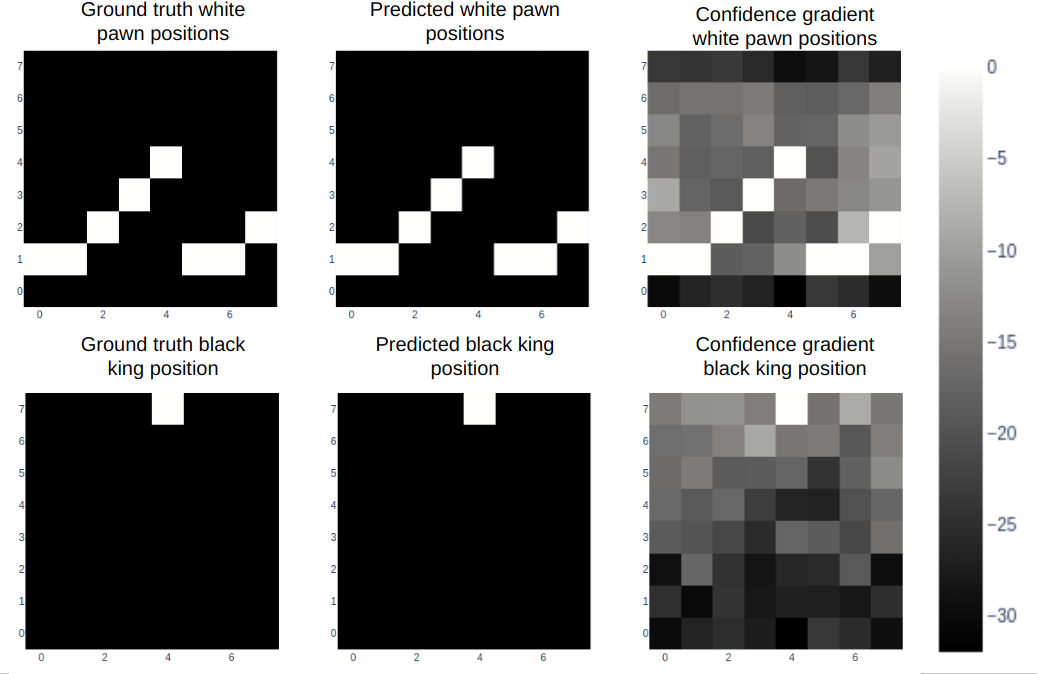
\includegraphics[width=0.85\textwidth]
        {figures/latent_space_analysis/probing_illustration.png}
    \caption[Probing analysis of a chess-playing language model.]{
        Probing analysis of an \glsfmtshort{llm} trained to play chess
        \parencite{karvonen2024emergentworldmodelslatent}.
    }
    \label{fig:probing_illustration}
\end{figure}

However, the fact that a concept can be decoded from \glspl{lr} does not necessarily imply that the model actually uses this information to perform its task.
To assess whether \glspl{lr} play a causal role in the model's output, it is possible to perform interventions on them.
An intervention consists of modifying a \gls{lr} in a controlled manner by activating or deactivating a given concept, and then studying its impact on the model's output.
If the resulting change in the model's output is consistent with the applied perturbation, this suggests that the representation had a causal role.

To this end, the \gls{lr} is minimally modified such that the probe prediction for the target concept $c_j$ changes state, while the predictions associated with other concepts remain unchanged.
This goal can be formulated as an optimization problem over the \gls{lr} itself.
The optimization is performed directly on the \gls{lr}, using \gls{sgd}.
The solution to this problem is the optimal modified \gls{lr}, defined as:
\[
\begin{aligned}
\latentRepresentation[l][*] =
\argmin_{\latentRepresentation[l][\prime]} \;
&\underbrace{\lambda_1 \, \mathcal{L}_{\mathrm{flip}}\big(\Probe{l}{j}(\latentRepresentation[l][\prime]), c_j\big)}_{\text{flip target concept } c_j} \\
+ \, &\underbrace{\lambda_2 \sum_{k \neq j} \mathcal{L}_{\mathrm{preserve}}\big(\Probe{l}{k}(\latentRepresentation[l][\prime]), c_k\big)}_{\text{preserve other concepts } c_{k \neq j}} \\
+ \, &\underbrace{\lambda_3 \|\latentRepresentation[l][\prime] - \latentRepresentation[l]\|_2^2}_{\text{minimality}},
\end{aligned}
\]
where:
\begin{itemize}
    \item $\latentRepresentation[l]$ is the original \gls{lr} of the input at layer $l$,
    \item $\latentRepresentation[l][\prime]$ is the modified \gls{lr} being optimized,
    \item $\latentRepresentation[l][*]$ is the optimal modified \gls{lr},
    \item $\mathcal{L}_{\mathrm{flip}}$: loss encouraging the prediction of the target concept $c_j$ to change state (i.e., flipping the predicted label),
    \item $\mathcal{L}_{\mathrm{preserve}}$: loss enforcing invariance of all non-target concepts $c_k$ for $k \neq j$,
    \item $\|\latentRepresentation[l][\prime] - \latentRepresentation[l]\|_2^2$: regularization term ensuring the modified \gls{lr} remains close to the original one,
    \item $\lambda_1, \lambda_2, \lambda_3$: weighting coefficients controlling the trade-off between the intervention strength, the preservation of other concepts, and the minimality of the perturbation.
\end{itemize}

In the context of \glspl{llm} studied previously, such interventions have been used to remove specific pieces from the model's internal representation of the game state \parencite{li2024emergentworldrepresentationsexploring, karvonen2024emergentworldmodelslatent}.
The main observation is that, in the vast majority of cases, the model behaves as if the piece had effectively disappeared.
The \gls{llm} continues to generate legal moves while correctly accounting for the absence of the removed piece.
This provides evidence for the causal role of these internal representations in the model's behavior.

A main limitation of the probing approach is that the concepts under investigation must be predefined before any analysis can be performed.
This introduces a strong bias.
Moreover, annotating a dataset for each concept is extremely time-consuming.
Interventions in \gls{ls} are also difficult to interpret, as it is not always clear what constitutes a meaningful change in the network's output under a given perturbation.

Finally, probing methods provide a binary view of concepts, focusing on whether a given concept is present or absent in a \gls{lr}.
This binary perspective can be restrictive, as concepts may be represented in a more continuous manner.

To obtain a more detailed characterization of these representations, the next section turns to methods that describe a concept as a direction in \gls{ls} along which it varies continuously.
\section{Directions}
\label{sec:latent_space_analysis_directions}

Probing describes a concept as a binary attribute, either present or absent in a \gls{lr}.
The methods in this section instead associate each concept with a direction in the \gls{ls}.
Moving a \gls{lr} along this direction is expected to strengthen or weaken the concept smoothly.
This provides information that a binary probe cannot express.

Empirically, it has been observed that shifting a \gls{lr} along such a direction can induce coherent and semantically meaningful changes in the model's output \parencite{haas2024discovering, voynov2020unsuperviseddiscoveryinterpretabledirections}.
Such a shift is a latent intervention (see Definition~\ref{def:latent_intervention}) and can be expressed mathematically as:
\begin{equationwhere}
\[
\latentRepresentation' = \latentRepresentation + \alpha \vect{v}_i,
\]
where:
\begin{itemize}
    \item $\latentRepresentation$ denotes the original \gls{lr},
    \item $\vect{v}_i$ is a unit vector associated with concept $i$,
    \item $\alpha$ controls the strength of the intervention,
    \item $\latentRepresentation'$ is the resulting perturbed \gls{lr}.
\end{itemize}
\end{equationwhere}

In many cases, the resulting change in the model's output varies smoothly with \(\alpha\), suggesting an approximately linear \gls{cs} with respect to certain semantic factors.
This observation has led to the hypothesis that neural representations may organize concepts in a partially linear manner within the \gls{ls}.

Vectors of this form are referred to as interpretable directions, as they correspond to transformations that can be associated with specific semantic attributes.
The objective of this line of work is therefore to identify directions in \gls{ls} that align with meaningful variations in the encoded concepts.
This is illustrated schematically in Figure~\ref{fig:latent_directions}, where arrows represent semantic shifts from one concept toward others, and moving along these directions induces a coherent change in the model's behavior, suggesting that the transition between concepts is continuously encoded along these axes.

\begin{figure}[t]
\centering

% ================================================================
%  latent_space_shared.tex
%  Couleurs, macros et styles partagés par toutes les figures
%  latent_space_*.tex
%  Usage : \input{figures/latent_space_analysis/latent_space_shared.tex}
% ================================================================

% ----------------------------------------------------------------
% Couleurs des clusters
% ----------------------------------------------------------------
\colorlet{colorA}{blue!70!cyan}
\colorlet{colorB}{orange}
\colorlet{colorC}{green!60!black}

% Couleurs de directions (latent_space_directions.tex)
\colorlet{colorDirBA}{violet}
\colorlet{colorDirBC}{red!70!black}

% ----------------------------------------------------------------
% Macros de dessin
% ----------------------------------------------------------------
\input{figures/latent_space_analysis/plot_points.tex}
\input{figures/latent_space_analysis/plot_ellipse.tex}
\input{figures/latent_space_analysis/plot_probe.tex}
\input{figures/latent_space_analysis/plot_direction.tex}

% ----------------------------------------------------------------
% Styles d'axe partagés
% ----------------------------------------------------------------
\pgfplotsset{
  % Axe standard (clustering, probing, directions)
  latent axis/.style={
    width=11cm,
    height=10cm,
    xmin=-7, xmax=8,
    ymin=-7, ymax=5.5,
    axis x line=bottom,
    axis y line=left,
    axis line style={
      -{Stealth[length=8pt, width=6pt]},
      thick
    },
    ticks=none,
    xlabel={},
    ylabel={},
    clip=true,
  },
  % Variante panneau carré (latent_space_sparse_autoencoders.tex)
  latent panel/.style={
    latent axis,
    width=9cm,
    height=9cm,
  },
  % Variante petit panneau (latent_space_embeddings.tex)
  % N.B. width/height sont passés explicitement par chaque fichier
  % via width=\lsePanelWd, height=\lsePanelHt dans l'axe.
  latent embed/.style={
    latent axis,
    every axis plot/.append style={forget plot},
  },
}


\resizebox{0.65\textwidth}{!}{
\begin{tikzpicture}
\begin{axis}[latent axis]

  % Point clouds
  \plotPoints[color=colorA, mark=*]{figures/latent_space_analysis/cluster_a.data}
  \plotPoints[color=colorB, mark=square*]{figures/latent_space_analysis/cluster_b.data}
  \plotPoints[color=colorC, size=2pt, mark=triangle*]{figures/latent_space_analysis/cluster_c.data}

  % Interpretable directions
  \plotProbe[color=colorDirBA, style=dashed, width=thick]{-11}{-31.5}
  \plotDirection[color=colorDirBA]{-2.5}{-4.0}{-3.0}{1.5}

  \plotProbe[color=colorDirBC, style=dashed, width=thick]{0.5224}{-2.694}
  \plotDirection[color=colorDirBC]{-2.5}{-4.0}{4.2}{-0.5}

  % Centroid B
  \fill[colorB] (axis cs:-2.5,-4.0) circle (4pt);

\end{axis}
\end{tikzpicture}
}

\caption{
    Interpretable directions in the \glsfmtshort{ls}.
}
\label{fig:latent_directions}
\end{figure}


This phenomenon has been extensively studied in generative image models.
Controlled perturbations of \glspl{lr} along interpretable directions can induce specific semantic transformations \parencite{voynov2020unsuperviseddiscoveryinterpretabledirections}.
Examples include stroke thickness modification in digit images, head rotation in facial images, and texture or background changes in natural images.
These transformations are illustrated in Figure~\ref{fig:interpretable_direction_illustration}, where each row corresponds to a distinct direction $\vect{v}_i$ and each column to an increasing value of $\alpha$.
These observations have led to the development of the field of \gls{ls} editing, whose objective is to manipulate generated content directly through modifications in \gls{ls} rather than through changes in the input prompt.

% figures/latent_space_analysis/interpretable_direction_illustration.tex

\begin{figure}[t]
    \centering
    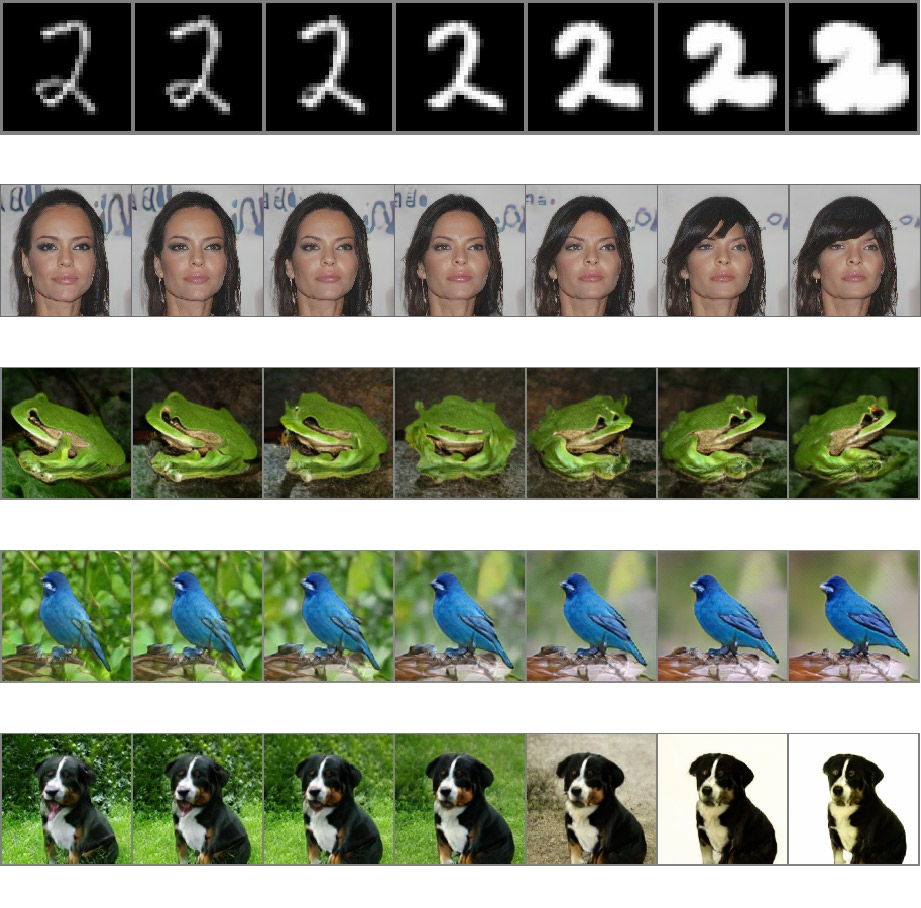
\includegraphics[width=0.85\textwidth]
        {figures/latent_space_analysis/interpretable_direction_illustration.png}
    \caption[Interpretable directions in the latent space of a generative model.]{
        Interpretable directions in the latent space of a generative model \parencite{voynov2020unsuperviseddiscoveryinterpretabledirections}.
    }
    \label{fig:interpretable_direction_illustration}
\end{figure}

A central challenge remains identifying such interpretable directions.
Most existing approaches rely on auxiliary models that encode human defined semantics, such as CLIP \parencite{haas2024discovering}, to relate latent variations to textual concepts.
Consequently, these methods inherit a limitation similar to that of probing techniques, since concept discovery depends on a pre-existing semantic framework defined by humans.

To overcome this limitation, a research direction known as unsupervised semantic discovery has emerged.
Its goal is to uncover interpretable directions in \gls{ls} without explicit semantic supervision.
In these approaches, one model applies perturbations along random directions in \gls{ls}, while a second model attempts to recognize the applied transformation.
If a stable correspondence emerges between the perturbation and its prediction, this suggests that the considered direction corresponds to a coherent \gls{cs} \parencite{voynov2020unsuperviseddiscoveryinterpretabledirections}.
In this framework, human intervention occurs only a posteriori, to verify whether the discovered directions indeed correspond to interpretable semantic variations.

Despite these advances, several challenges remain.
It appears that not all concepts encoded by \glspl{nn} are linearly identifiable in \gls{ls}.
In addition, \glspl{lr} often exhibit a phenomenon known as entanglement, illustrated in Figure~\ref{fig:entanglement_illustration}, where multiple semantic attributes are mixed within the same directions of the \gls{ls}.
For instance, in a generative face model, moving along the \enquote{glasses} direction may simultaneously modify age and gender, whereas a disentangled \gls{lr} would let each axis control a single semantic attribute while leaving the others unchanged.

This lack of separability suggests that semantic information is not cleanly organized in the \gls{ls}.
This observation motivates the \SuperpositionHypothesisName, which proposes a different view of how \glspl{nn} organize information internally.
The next section introduces this hypothesis.

\begin{figure}[t]
    \centering
    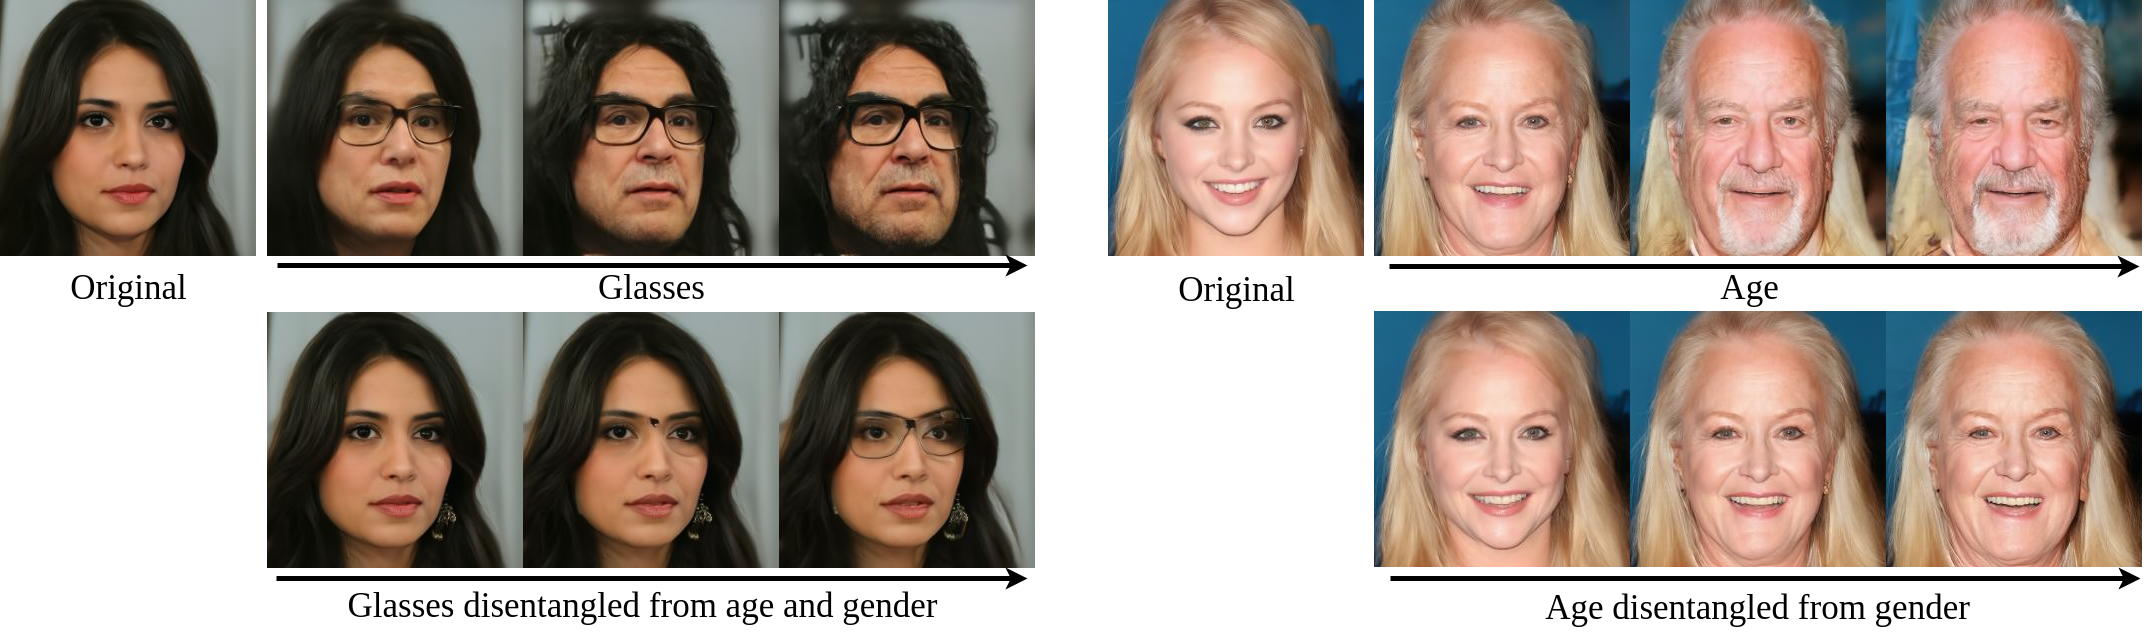
\includegraphics[width=0.85\textwidth]
        {figures/latent_space_analysis/entanglement_illustration.png}
    \caption[Entanglement in the latent space of a generative face model.]{
        Illustration of entanglement in the latent space of a generative face
        model \parencite{haas2024discovering}.
    }
    \label{fig:entanglement_illustration}
\end{figure}
\section{Superposition}
\label{sec:latent_space_analysis_superposition}

The previous section highlighted a limitation of interpretable directions.
Only a limited number of concepts can be represented by a linear direction, and these directions are often entangled with multiple semantic concepts.
To account for this, an extension of the \ConceptHypothesisName has been proposed under the name \SuperpositionHypothesisName, formalized in Hypothesis~\ref{hyp:superposition} \parencite{elhage2022superposition}.

\begin{hypothesis}{Superposition Hypothesis}{superposition}
Concepts are preferentially represented by distinct linear directions in \gls{ls}.
When the number of concepts exceeds the available dimensions, multiple concepts are encoded in superposition within the same directions.
\end{hypothesis}

According to this hypothesis, in an unconstrained \gls{ls}, each concept is represented in its own independent linear direction.
The idealized non-superposed \gls{lr} can be mathematically expressed as follows:
\[
\latentRepresentation = \sum_{i=1}^{n} \alpha_i \vect{v}_i,
\qquad
\forall i \neq j,\quad \vect{v}_i^\top \vect{v}_j \approx 0,
\qquad
\|\boldsymbol{\alpha}\|_0 \ll n,
\]

where:
\begin{itemize}
    \item $\latentRepresentation$ denotes a \gls{lr},
    \item $n$ is the total number of concepts,
    \item $\vect{v}_i$ represents the direction associated with concept $c_i$,
    \item $\alpha_i$ corresponds to the activation strength of concept $c_i$ in the \gls{lr} $\latentRepresentation$,
    \item $\vect{v}_i^\top \vect{v}_j \approx 0$ indicates that concept directions are approximately orthogonal, meaning each concept independently controls a single factor of variation,
    \item $\|\boldsymbol{\alpha}\|_0 \ll n$ indicates that only a small fraction of concepts are active for a given \gls{lr}.
\end{itemize}

However, \glspl{nn} operate in finite-dimensional spaces, so when the number of concepts exceeds the available dimensions, such a one-to-one correspondence becomes impractical.
The network must therefore reuse its representational dimensions, allowing multiple concepts to be encoded using the same directions.
This shared encoding is referred to as superposition \parencite{bricken2023monosemanticity}.
This phenomenon becomes an obstacle for any method that attempts to analyze \glspl{lr} directly in the original activation space.

Building on this observation, several works based on the \SuperpositionHypothesisName have developed methods that aim to recover less superposed \glspl{lr}.
A common approach is to map \gls{ls} into a higher-dimensional space while imposing additional constraints that encourage individual concepts to be represented separately.
This transformation is illustrated in Figure~\ref{fig:dense_to_sparse_sae}, while \glspl{lr} are entangled in the initial \gls{ls}, the sparse representation aligns each concept with a dedicated feature axis.

\providecommand{\lsePanelWidth}{6cm}
\newlength{\saePanelWd}
\newlength{\saePanelHt}
\newlength{\saePanelGap}

% Lengths must be set BEFORE \resizebox so pgfplots sees non-zero values.
\setlength{\saePanelWd}{\lsePanelWidth}
\pgfmathsetlength{\saePanelHt} {\saePanelWd * 5 / 6}
\pgfmathsetlength{\saePanelGap}{\saePanelWd * 0.9}

\begin{figure}[t]
\centering

% ================================================================
%  latent_space_shared.tex
%  Couleurs, macros et styles partagés par toutes les figures
%  latent_space_*.tex
%  Usage : \input{figures/latent_space_analysis/latent_space_shared.tex}
% ================================================================

% ----------------------------------------------------------------
% Couleurs des clusters
% ----------------------------------------------------------------
\colorlet{colorA}{blue!70!cyan}
\colorlet{colorB}{orange}
\colorlet{colorC}{green!60!black}

% Couleurs de directions (latent_space_directions.tex)
\colorlet{colorDirBA}{violet}
\colorlet{colorDirBC}{red!70!black}

% ----------------------------------------------------------------
% Macros de dessin
% ----------------------------------------------------------------
\input{figures/latent_space_analysis/plot_points.tex}
\input{figures/latent_space_analysis/plot_ellipse.tex}
\input{figures/latent_space_analysis/plot_probe.tex}
\input{figures/latent_space_analysis/plot_direction.tex}

% ----------------------------------------------------------------
% Styles d'axe partagés
% ----------------------------------------------------------------
\pgfplotsset{
  % Axe standard (clustering, probing, directions)
  latent axis/.style={
    width=11cm,
    height=10cm,
    xmin=-7, xmax=8,
    ymin=-7, ymax=5.5,
    axis x line=bottom,
    axis y line=left,
    axis line style={
      -{Stealth[length=8pt, width=6pt]},
      thick
    },
    ticks=none,
    xlabel={},
    ylabel={},
    clip=true,
  },
  % Variante panneau carré (latent_space_sparse_autoencoders.tex)
  latent panel/.style={
    latent axis,
    width=9cm,
    height=9cm,
  },
  % Variante petit panneau (latent_space_embeddings.tex)
  % N.B. width/height sont passés explicitement par chaque fichier
  % via width=\lsePanelWd, height=\lsePanelHt dans l'axe.
  latent embed/.style={
    latent axis,
    every axis plot/.append style={forget plot},
  },
}


\resizebox{1\textwidth}{!}{
\begin{tikzpicture}

  % ================================================================
  % LEFT PANEL — Dense latent space
  % ================================================================
  \begin{scope}[xshift=0pt]
  \begin{axis}[
    name=axisLeft,
    latent embed,
    width=\saePanelWd,
    height=\saePanelHt,
    xmin=-7, xmax=8,
    ymin=-7, ymax=5.5,
  ]
    \plotPoints[color=colorA, mark=*]{figures/latent_space_analysis/cluster_a.data}
    \plotPoints[color=colorB, mark=square*]{figures/latent_space_analysis/cluster_b.data}
    \plotPoints[color=colorC, size=2pt, mark=triangle*]{figures/latent_space_analysis/cluster_c.data}
    \end{axis}
    \node[anchor=north, yshift=-6pt] at (axisLeft.south)
      {(a) Dense latent space};
  \end{scope}

  % ================================================================
  % RIGHT PANEL — Sparse SAE space
  % ================================================================
  \begin{scope}[xshift=\saePanelGap]
  \begin{axis}[
    name=axisRight,
    width=\saePanelWd,
    height=\saePanelHt,
    xmin=-8.5, xmax=8.5,
    ymin=-6,   ymax=9,
    axis lines=none,
    ticks=none,
    clip=true,
  ]

    \draw[colorA, thick, -{Stealth[length=7pt,width=5pt]}]
      (axis cs:0,0) -- (axis cs:0,7);
    \node[colorA, font=\small\bfseries, above] at (axis cs:0,7.3)
      {Feature $A$};

    \draw[colorB, thick, -{Stealth[length=7pt,width=5pt]}]
      (axis cs:0,0) -- (axis cs:-6.062,-3.5);
    \node[colorB, font=\small\bfseries, below left] at (axis cs:-6.062,-3.8)
      {Feature $B$};

    \draw[colorC, thick, -{Stealth[length=7pt,width=5pt]}]
      (axis cs:0,0) -- (axis cs:6.062,-3.5);
    \node[colorC, font=\small\bfseries, below right] at (axis cs:6.062,-3.8)
      {Feature $C$};

    \plotPoints[color=colorA, mark=*]{figures/latent_space_analysis/sae_right_a.data}
    \plotPoints[color=colorB, mark=square*]{figures/latent_space_analysis/sae_right_b.data}
    \plotPoints[color=colorC, size=2pt, mark=triangle*]{figures/latent_space_analysis/sae_right_c.data}

  \end{axis}
  \node[anchor=north, yshift=-6pt] at (axisRight.south)
    {(b) Sparse SAE space};
  \end{scope}

\end{tikzpicture}
}

\caption[Transformation from a dense to a sparse \glsfmtshort{ls}.]{
  Transformation from a dense \glsfmtshort{ls}~(a) to a sparse
  \glsfmtshort{sae} representation~(b).
}
\label{fig:dense_to_sparse_sae}
\end{figure}


\glspl{sae} provide a practical implementation of this approach and can be defined as follows:
\[
\vect{z} = \Encoder(\latentRepresentation), \quad \hat{\latentRepresentation} = \Decoder(\vect{z})
\]
\[
\mathcal{L}_{\mathrm{auto}} = \|\latentRepresentation - \hat{\latentRepresentation}\|_2^2 + \lambda \|\vect{z}\|_1
\]

where:
\begin{itemize}
    \item $\Encoder(\latentRepresentation)$ is the encoding function that projects the original \gls{lr} $\latentRepresentation$ into a higher-dimensional sparse space,
    \item $\Decoder(\vect{z})$ is the decoding function that reconstructs the original \gls{lr} from the sparse code,
    \item $\vect{z} \in \mathcal{Z}$ is the sparse representation of $\latentRepresentation$, with $\dim(\vect{z}) \gg \dim(\latentRepresentation)$,
    \item $\hat{\latentRepresentation}$ is the reconstructed \gls{lr},
    \item $\|\latentRepresentation - \hat{\latentRepresentation}\|_2^2$ is the reconstruction loss ensuring that the original \gls{lr} can be faithfully recovered,
    \item $\|\vect{z}\|_1$ is the sparsity regularization term that encourages most components of $\vect{z}$ to be zero,
    \item $\lambda$ is a weighting coefficient controlling the trade-off between reconstruction fidelity and sparsity.
\end{itemize}

The parameters of these projection functions $\Encoder$ and $\Decoder$ are learned by minimizing $\mathcal{L}_{\mathrm{auto}}$ using \gls{sgd}.
Under this formulation, each dimension of $\mathcal{Z}$ is interpreted as a dedicated concept direction.

In practice, both $\Encoder$ and $\Decoder$ are implemented as linear projections between the original \gls{ls} and the high-dimensional space $\mathcal{Z}$. This choice is motivated by the same principle underlying probing methods. The transformation applied to the \gls{lr} should remain as simple as possible.
Using more expressive projection functions could introduce additional structures into the transformed \gls{lr}. In this case, it would become difficult to determine whether an observed concept was already encoded in the model's \gls{lr}, or whether it was introduced by the projection itself. Restricting $\Encoder$ and $\Decoder$ to linear projections therefore helps ensure that the concepts identified in $\mathcal{Z}$ can be attributed to the original \gls{lr}, rather than to the transformation used to analyze it.

The method proves to be powerful when successfully applied to language models \parencite{templeton2024scaling}.
In these applications, \glspl{sae} are used to desuperpose the \gls{lr} of \glspl{llm}.
Once this \gls{lr} is obtained, it has been shown that many concept vectors exhibit semantic properties.
A example is the Golden Gate Bridge concept direction, illustrated in Figure~\ref{fig:sparse_autoencoder_illustration}, which activates systematically whenever the input text or image refers to the Golden Gate Bridge, regardless of the language or modality.
This demonstrates that the learned concept is not tied to a specific surface form but captures a deeper semantic abstraction shared across modalities.

\begin{figure}[t]
    \centering
    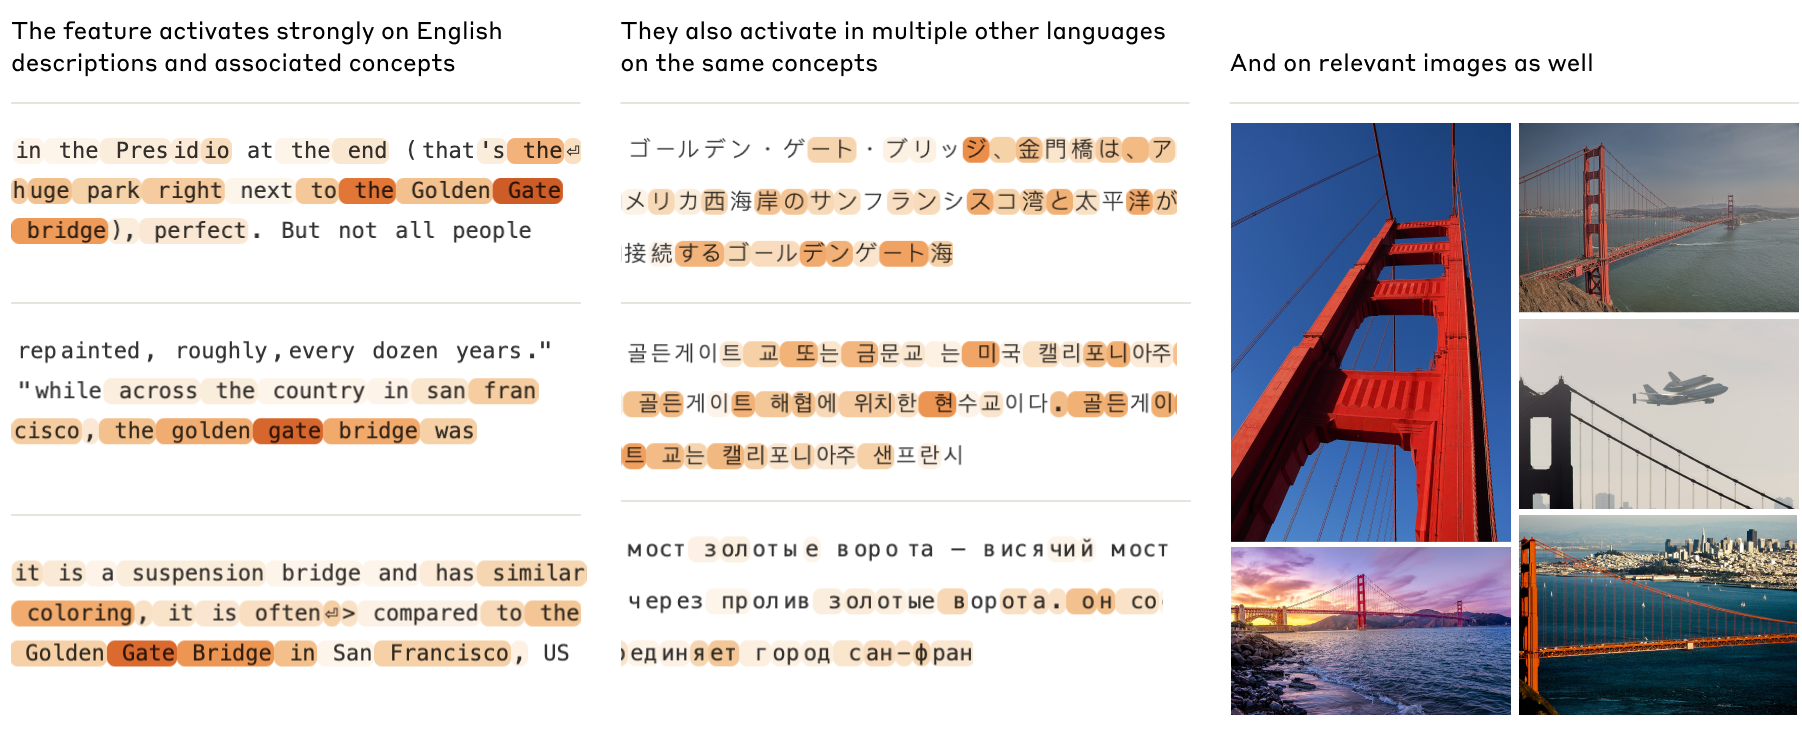
\includegraphics[width=0.85\textwidth]
        {figures/latent_space_analysis/sparse_autoencoder_illustration.png}
    \caption[The Golden Gate Bridge concept direction of an \glsfmtshort{sae}.]{
        A concept direction corresponding to the Golden Gate Bridge, discovered
        by an \glsfmtshort{sae} applied to an \glsfmtshort{llm}
        \parencite{templeton2024scaling}.
    }
    \label{fig:sparse_autoencoder_illustration}
\end{figure}

\glspl{sae} also provide a way to intervene directly on the \gls{lr} learned by the model.
A concept can be artificially activated by modifying its corresponding feature in the sparse representation $\vect{z}$, even when the input contains no reference to it.
The modified \gls{lr} is then projected back into the original activation space, after which the model proceeds with standard next-token generation from $\latentRepresentation^{*}$:
\[
\latentRepresentation^{*} = \Decoder(\vect{z}^*), \quad \text{where} \quad \vect{z}^* = \vect{z} + \alpha \, \vect{e}^{(i)},
\]

where:
\begin{itemize}
    \item $\vect{z}$ is the original sparse representation of the input,
    \item $\vect{z}^*$ is the modified sparse representation,
    \item $\vect{e}^{(i)}$ is the basis vector of $\mathcal{Z}$ associated with the target concept direction,
    \item $\alpha$ controls the strength of the artificial activation,
    \item $\latentRepresentation^{*}$ is the resulting edited \gls{lr} in the original activation space.
\end{itemize}

With this method, a reference to the Golden Gate Bridge can be injected into the \gls{llm}'s internal representation.
This causes the model's output to shift toward discussing the Golden Gate Bridge, even when the prompt contains no reference to it.
This provides evidence that the learned feature plays a causal role in the model's behavior.
Such interventions enable control over specific model behaviors through \gls{ls} editing.

Despite their empirical success, \SuperpositionHypothesisName exhibit several important limitations that question their assumptions. 
These limitations can be summarized as follows:
\begin{itemize}
    \item \textbf{Instability of the decomposition.}
    Repeating the \gls{sae} training process multiple times on the same model does not yield the same decomposition of the \gls{ls}.
    Different runs produce different concept directions in $\mathcal{Z}$, even when achieving comparable reconstruction performance, which raises questions about the reliability of the discovered \glspl{cs}.

    \item \textbf{Lack of semantic coverage.}
    In the high-dimensional space $\mathcal{Z}$, a large fraction of dimensions do not correspond to any interpretable semantic concept.
    This abundance of non-semantic directions raises questions about whether the decomposition truly reflects the model's \glspl{cs}.

    \item \textbf{Sparsity--semantics trade-off.}
    Increasing the sparsity coefficient $\lambda$ beyond a certain threshold degrades the semantic quality of the learned features \parencite{tanhPenaltyDictionaryLearning}.
    Suggesting that enforcing excessive sparsity comes at the cost of interpretability.

    \item \textbf{Failure of scaling to remove superposition.}
    Under the \SuperpositionHypothesisName, increasing the dimensionality of the \gls{ls} should reduce superposition.
    However, this is not observed in practice.
    Even in very high-dimensional \glspl{ls}, representations remain superposed, indicating that scaling alone does not resolve the entanglement.
\end{itemize}

These limitations suggest that \SuperpositionHypothesisName, while powerful, do not fully resolve the problem of \gls{cs}.
Convincing empirical results do not necessarily validate the underlying theoretical assumptions.

So far, every method described, whether based on probing, interpretable directions, or superposition, relies on a common assumption.
The \gls{cs} can be recovered from \glspl{lr} through a linear decomposition.
This assumption has enabled substantial progress in understanding neural representations, but it also imposes a strong constraint on how concepts are expected to be represented.
The following section examines clustering as an alternative approach that does not rely on this assumption.
\section{Clustering}
\label{sec:latent_space_analysis_clustering}

As the previous section noted, every \gls{ls} analysis method presented so far rests on a linear view of the \gls{cs}.
For probing methods, concepts must be at least partially linearly separable for simple probes to detect them.
Interpretable direction methods posit that variations associated with a concept can be captured by moving along a linear axis of the \gls{ls}.
The \SuperpositionHypothesisName proposes that concepts are represented through linear directions that become entangled because of representational capacity constraints.

Although these assumptions have led to empirical successes, several observations suggest that the linearity hypothesis may not fully capture the \gls{cs}.
For instance, some concepts can only be recovered using non-linear probes.
Likewise, methods based on interpretable directions typically identify only a limited number of semantic factors.
Finally, in \gls{sae} approaches, enforcing excessive sparsity degrades interpretability.
This suggests that the underlying representation may not be perfectly described by a sparse linear decomposition.
Taken together, these observations indicate that semantic concepts may not always exhibit a linear \gls{cs}.
This motivates the exploration of alternative approaches that rely on weaker assumptions regarding the geometry of \glspl{ls}.

To the best of our knowledge, clustering-based analysis is the only family of \gls{ls} analysis methods that does not rely on any assumption of a linear \gls{cs} \parencite{ren_deep_2022, wei_overview_2024}.
Rather than assuming that concepts correspond to directions, clustering methods only assume that conceptual similar inputs produce nearby \glspl{lr}.
Conversely, inputs that differ significantly from a concept perspective are expected to be located farther apart in the \gls{ls}.
This is a considerably weaker assumption, in the sense that it is empirically verified in a wide range of settings.

Under this assumption, the discovery of concepts can be reformulated as the identification of groups of \glspl{lr} that occupy the same region of the \gls{ls}.
This is shown schematically in Figure~\ref{fig:latent_clusters}, where the points represent \glspl{lr} associated with concepts, and the ellipses indicate the approximate extent of each group and highlight their geometric separation.

\begin{figure}[t]
\centering

% ================================================================
%  latent_space_shared.tex
%  Couleurs, macros et styles partagés par toutes les figures
%  latent_space_*.tex
%  Usage : \input{figures/latent_space_analysis/latent_space_shared.tex}
% ================================================================

% ----------------------------------------------------------------
% Couleurs des clusters
% ----------------------------------------------------------------
\colorlet{colorA}{blue!70!cyan}
\colorlet{colorB}{orange}
\colorlet{colorC}{green!60!black}

% Couleurs de directions (latent_space_directions.tex)
\colorlet{colorDirBA}{violet}
\colorlet{colorDirBC}{red!70!black}

% ----------------------------------------------------------------
% Macros de dessin
% ----------------------------------------------------------------
\input{figures/latent_space_analysis/plot_points.tex}
\input{figures/latent_space_analysis/plot_ellipse.tex}
\input{figures/latent_space_analysis/plot_probe.tex}
\input{figures/latent_space_analysis/plot_direction.tex}

% ----------------------------------------------------------------
% Styles d'axe partagés
% ----------------------------------------------------------------
\pgfplotsset{
  % Axe standard (clustering, probing, directions)
  latent axis/.style={
    width=11cm,
    height=10cm,
    xmin=-7, xmax=8,
    ymin=-7, ymax=5.5,
    axis x line=bottom,
    axis y line=left,
    axis line style={
      -{Stealth[length=8pt, width=6pt]},
      thick
    },
    ticks=none,
    xlabel={},
    ylabel={},
    clip=true,
  },
  % Variante panneau carré (latent_space_sparse_autoencoders.tex)
  latent panel/.style={
    latent axis,
    width=9cm,
    height=9cm,
  },
  % Variante petit panneau (latent_space_embeddings.tex)
  % N.B. width/height sont passés explicitement par chaque fichier
  % via width=\lsePanelWd, height=\lsePanelHt dans l'axe.
  latent embed/.style={
    latent axis,
    every axis plot/.append style={forget plot},
  },
}


\resizebox{0.65\textwidth}{!}{
\begin{tikzpicture}
\begin{axis}[latent axis]

  % Cluster boundaries
  \plotEllipse[color=colorA, width=very thick, fill=colorA, fillopacity=0.08]
    {-3}{1.5}{15}{2.3}{1.2}
  \plotEllipse[color=colorB, width=very thick, fill=colorB, fillopacity=0.08]
    {-2.5}{-4}{10}{2.2}{1.1}
  \plotEllipse[color=colorC, width=very thick, fill=colorC, fillopacity=0.08]
    {4.2}{-0.5}{-20}{1.4}{2.6}

  % Point clouds
  \plotPoints[color=colorA, mark=*]{figures/latent_space_analysis/cluster_a.data}
  \plotPoints[color=colorB, mark=square*]{figures/latent_space_analysis/cluster_b.data}
  \plotPoints[color=colorC, size=2pt, mark=triangle*]{figures/latent_space_analysis/cluster_c.data}

\end{axis}
\end{tikzpicture}
}

\caption{
  Visualization of the \glsfmtshort{ls} structure.
}
\label{fig:latent_clusters}
\end{figure}


This idea forms the basis of the research field known as deep clustering.
In these approaches, a collection of inputs is projected into a \gls{ls} using a \gls{nn}.
The resulting \glspl{lr} form a point cloud on which standard clustering algorithms can be applied.
The obtained clusters are then interpreted as representing distinct concepts.

Deep clustering has been particularly successful in unsupervised image classification.
For this type of task, a specific \gls{nn} architecture called an autoencoder is commonly used.
An autoencoder is composed of an encoder $\Encoder$ and a decoder $\Decoder$.
The encoder maps an input $\vect{x} \in \mathcal{X}$ to a low-dimensional \gls{lr} $\vect{z} \in \mathbb{R}^d$, the \gls{lr} produced by the encoder.
The decoder then maps this \gls{lr} back to the input space to produce a reconstruction $\hat{\vect{x}}$.

The model is trained by \gls{sgd} to minimize the reconstruction error between the original input and its reconstruction using a \gls{mse} loss.
This objective encourages the \gls{ls} to preserve the most informative features of the input while enforcing a compact representation.
This can be expressed mathematically as follows:
\[
\vect{x}
\xrightarrow{\;\Encoder\;}
\vect{z}
\xrightarrow{\;\Decoder\;}
\hat{\vect{x}},
\qquad
d \ll \dim(\mathcal{X}),
\qquad
\mathcal{L}_{\mathrm{rec}}
=
\frac{1}{N}\sum_{i=1}^{N}
\left\|\vect{x}^{(i)}-\hat{\vect{x}}^{(i)}\right\|_2^2.
\]

Once the autoencoder has been trained sufficiently well, the reconstruction loss $\mathcal{L}_{\mathrm{rec}}$ should be low enough for the learned representation to be useful.
A clustering algorithm can then be applied to the compressed representations of the images.
Let $\mathcal{D}$ denote a dataset of inputs, through the encoder $\Encoder$, this dataset is mapped to a point cloud in the \gls{ls}:
\[
\mathcal{Z} = \{\vect{z}^{(i)} \in \mathbb{R}^d \mid \vect{z}^{(i)} = \Encoder(\vect{x}^{(i)}), \; \vect{x}^{(i)} \in \mathcal{D} \}.
\]

A classical clustering algorithm is applied to the set $\mathcal{Z}$ of \glspl{lr} to identify groups of similar \glspl{lr}.
Each resulting cluster can therefore be interpreted as a group of images that the model considers similar.

An example of this methodology can be observed in Figure~\ref{fig:deep_clustering_illustration}, where the approach is applied to the STL-10 dataset \parencite{coates2011analysis} using $k$-means clustering \parencite{macqueen1967multivariate} with a number of clusters arbitrarily fixed to $K = 10$ \parencite{xie_unsupervised_2016}.
For each cluster, the corresponding line shows the $10$ samples closest to the associated centroid in the \gls{ls}.
We observe that the method captures coherent semantic categories such as animals, vehicles, and flying entities.

\begin{figure}[t]
    \centering
    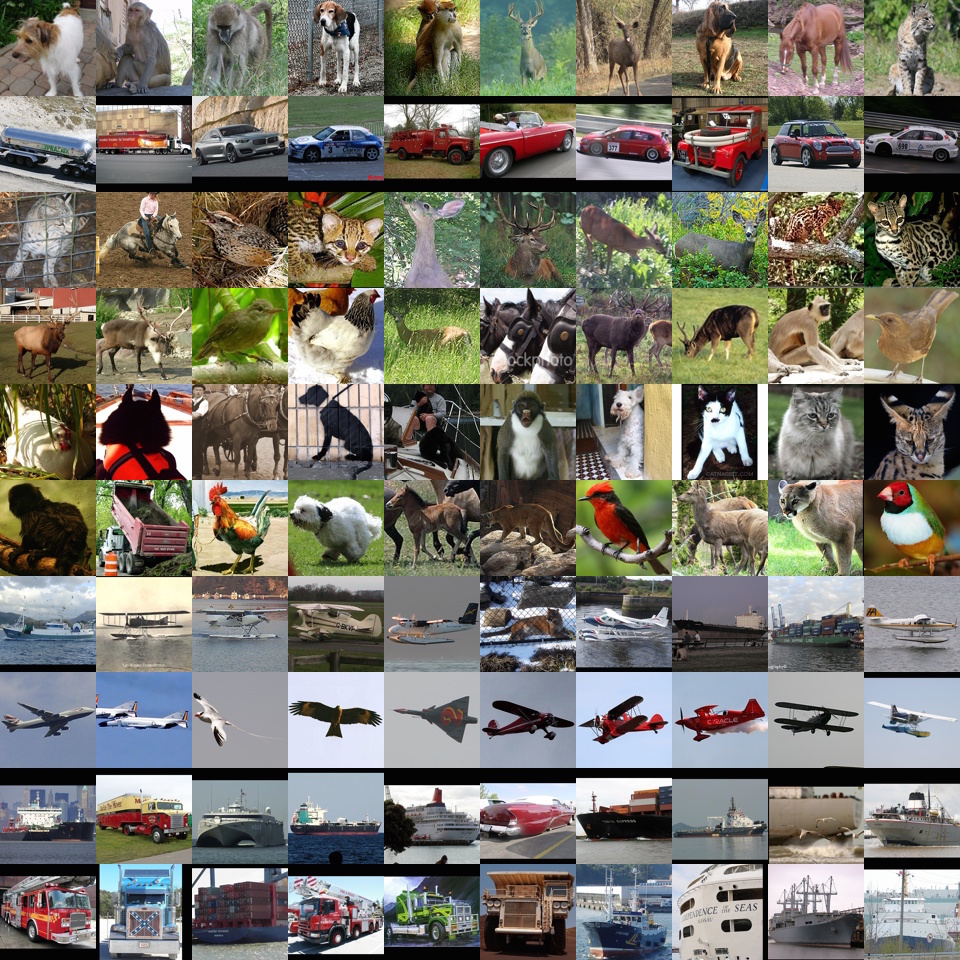
\includegraphics[width=0.85\textwidth]
        {figures/latent_space_analysis/deep_clustering_illustration.jpg}
    \caption[Clusters discovered by deep clustering on natural images.]{
        Clusters discovered by a deep clustering model applied to natural images \parencite{xie_unsupervised_2016}.
    }
    \label{fig:deep_clustering_illustration}
\end{figure}

This result is particularly striking given that the only available information to the system consists of raw images.
It suggests that the compression process induces a \gls{ls} in which semantically meaningful \glspl{cs} emerge.

More advanced approaches combine representation learning and clustering within a single optimization process.
In this setting, additional loss terms encourage \glspl{lr} to organize themselves around cluster centroids during training.
This often produces \glspl{ls} that are easier to analyze and improves the quality of the discovered semantic \glspl{cs} \parencite{guo_improved_2017, miklautz_breaking_2024}.

Clustering-based analysis presents several important limitations.
First, as with most unsupervised semantic discovery techniques, interpreting the resulting clusters remains partly subjective.
Benchmark datasets often provide class labels for evaluation, but the discovered clusters may not match the categories that humans consider relevant. 

Second, clustering methods are highly sensitive to design choices.
The number of clusters, the distance metric, and the clustering algorithm itself can all significantly influence the results.
Parameter selection is therefore challenging and often requires substantial empirical tuning.

Finally, to the best of our knowledge, no intervention technique has yet been proposed in the context of clustering-based analysis.
Unlike probing or \gls{sae} analysis, which allow targeted modifications of \glspl{lr} to study their causal role, clustering methods currently offer no mechanism to alter the model's behavior by acting directly on the discovered \glspl{cs}.

\section{Conclusion}
\label{sec:latent_space_analysis_conclusion}

% figures/latent_space_analysis/latent_space_overview.tex

\providecommand{\lsePanelWidth}{5.5cm}
\newlength{\ovPanelWd}
\newlength{\ovPanelHt}
\newlength{\ovPanelGap}
\newlength{\ovRowGap}

\setlength{\ovPanelWd}{\lsePanelWidth}
\pgfmathsetlength{\ovPanelHt} {\ovPanelWd * 5 / 6}
\pgfmathsetlength{\ovPanelGap}{\ovPanelWd * 1}
\pgfmathsetlength{\ovRowGap}  {\ovPanelHt * 1}

\begin{figure}[t]
\centering

% ================================================================
%  latent_space_shared.tex
%  Couleurs, macros et styles partagés par toutes les figures
%  latent_space_*.tex
%  Usage : \input{figures/latent_space_analysis/latent_space_shared.tex}
% ================================================================

% ----------------------------------------------------------------
% Couleurs des clusters
% ----------------------------------------------------------------
\colorlet{colorA}{blue!70!cyan}
\colorlet{colorB}{orange}
\colorlet{colorC}{green!60!black}

% Couleurs de directions (latent_space_directions.tex)
\colorlet{colorDirBA}{violet}
\colorlet{colorDirBC}{red!70!black}

% ----------------------------------------------------------------
% Macros de dessin
% ----------------------------------------------------------------
\input{figures/latent_space_analysis/plot_points.tex}
\input{figures/latent_space_analysis/plot_ellipse.tex}
\input{figures/latent_space_analysis/plot_probe.tex}
\input{figures/latent_space_analysis/plot_direction.tex}

% ----------------------------------------------------------------
% Styles d'axe partagés
% ----------------------------------------------------------------
\pgfplotsset{
  % Axe standard (clustering, probing, directions)
  latent axis/.style={
    width=11cm,
    height=10cm,
    xmin=-7, xmax=8,
    ymin=-7, ymax=5.5,
    axis x line=bottom,
    axis y line=left,
    axis line style={
      -{Stealth[length=8pt, width=6pt]},
      thick
    },
    ticks=none,
    xlabel={},
    ylabel={},
    clip=true,
  },
  % Variante panneau carré (latent_space_sparse_autoencoders.tex)
  latent panel/.style={
    latent axis,
    width=9cm,
    height=9cm,
  },
  % Variante petit panneau (latent_space_embeddings.tex)
  % N.B. width/height sont passés explicitement par chaque fichier
  % via width=\lsePanelWd, height=\lsePanelHt dans l'axe.
  latent embed/.style={
    latent axis,
    every axis plot/.append style={forget plot},
  },
}


\resizebox{\textwidth}{!}{
\begin{tikzpicture}

  % ============================================================
  % (a) TOP-LEFT — Probing
  % ============================================================
  \begin{scope}[xshift=0pt, yshift=0pt]
  \begin{axis}[
    name=axisProbing,
    latent embed, width=\ovPanelWd, height=\ovPanelHt,
  ]
    \fill[colorA, opacity=0.10]
      (axis cs:-7,-4) -- (axis cs:-7,5.5) -- (axis cs:2.5,5.5) -- cycle;
    \fill[colorB, opacity=0.10]
      (axis cs:-7,0.1) -- (axis cs:8,-4.4) --
      (axis cs:8,-7)   -- (axis cs:-7,-7)  -- cycle;
    \fill[colorC, opacity=0.10]
      (axis cs:-0.75,5.5) -- (axis cs:8,5.5) --
      (axis cs:8,-7)      -- (axis cs:5.5,-7) -- cycle;
    \plotProbe[color=colorA]{1}{3}
    \plotProbe[color=colorB]{-0.3}{-2}
    \plotProbe[color=colorC]{-2}{4}
    \plotPoints[color=colorA, mark=*]{figures/latent_space_analysis/cluster_a.data}
    \plotPoints[color=colorB, mark=square*]{figures/latent_space_analysis/cluster_b.data}
    \plotPoints[color=colorC, size=2pt, mark=triangle*]{figures/latent_space_analysis/cluster_c.data}
  \end{axis}
  \node[anchor=north, yshift=-6pt] at (axisProbing.south)
    {\textbf{(a)} Probing};
  \end{scope}

  % ============================================================
  % (b) TOP-RIGHT — Directions
  % ============================================================
  \begin{scope}[xshift=\ovPanelGap, yshift=0pt]
  \begin{axis}[
    name=axisDirections,
    latent embed, width=\ovPanelWd, height=\ovPanelHt,
  ]
    \plotPoints[color=colorA, mark=*]{figures/latent_space_analysis/cluster_a.data}
    \plotPoints[color=colorB, mark=square*]{figures/latent_space_analysis/cluster_b.data}
    \plotPoints[color=colorC, size=2pt, mark=triangle*]{figures/latent_space_analysis/cluster_c.data}
    \plotProbe[color=colorDirBA, style=dashed, width=thick]{-11}{-31.5}
    \plotDirection[color=colorDirBA]{-2.5}{-4.0}{-3.0}{1.5}
    \plotProbe[color=colorDirBC, style=dashed, width=thick]{0.5224}{-2.694}
    \plotDirection[color=colorDirBC]{-2.5}{-4.0}{4.2}{-0.5}
    \fill[colorB] (axis cs:-2.5,-4.0) circle (4pt);
  \end{axis}
  \node[anchor=north, yshift=-6pt] at (axisDirections.south)
    {\textbf{(b)} Directions};
  \end{scope}

  % ============================================================
  % (c) BOTTOM-LEFT — Superposition
  % ============================================================
  \begin{scope}[xshift=0pt, yshift=-\ovRowGap]
  \begin{axis}[
    name=axisSAE,
    width=\ovPanelWd, height=\ovPanelHt,
    xmin=-8.5, xmax=8.5, ymin=-6, ymax=9,
    axis lines=none, ticks=none, clip=true,
  ]
    \draw[colorA, thick, -{Stealth[length=5pt,width=4pt]}]
      (axis cs:0,0) -- (axis cs:0,7);
    \node[colorA, font=\small\bfseries, above] at (axis cs:0,7.2) {$A$};
    \draw[colorB, thick, -{Stealth[length=5pt,width=4pt]}]
      (axis cs:0,0) -- (axis cs:-6.062,-3.5);
    \node[colorB, font=\small\bfseries, below left] at (axis cs:-6.062,-3.7) {$B$};
    \draw[colorC, thick, -{Stealth[length=5pt,width=4pt]}]
      (axis cs:0,0) -- (axis cs:6.062,-3.5);
    \node[colorC, font=\small\bfseries, below right] at (axis cs:6.062,-3.7) {$C$};
    \plotPoints[color=colorA, mark=*]{figures/latent_space_analysis/sae_right_a.data}
    \plotPoints[color=colorB, mark=square*]{figures/latent_space_analysis/sae_right_b.data}
    \plotPoints[color=colorC, size=2pt, mark=triangle*]{figures/latent_space_analysis/sae_right_c.data}
  \end{axis}
  \node[anchor=north, yshift=-6pt] at (axisSAE.south)
    {\textbf{(c)} Superposition};
  \end{scope}

% ============================================================
  % (d) BOTTOM-RIGHT — Clustering
  % ============================================================
  \begin{scope}[xshift=\ovPanelGap, yshift=-\ovRowGap]
  \begin{axis}[
    name=axisClustering,
    latent embed, width=\ovPanelWd, height=\ovPanelHt,
  ]
    \plotEllipse[color=colorA, width=very thick, fill=colorA, fillopacity=0.08]
      {-3}{1.5}{15}{1.4}{0.8}
    \plotEllipse[color=colorB, width=very thick, fill=colorB, fillopacity=0.08]
      {-2.5}{-4}{10}{1.3}{0.7}
    \plotEllipse[color=colorC, width=very thick, fill=colorC, fillopacity=0.08]
      {4.2}{-0.5}{-20}{0.9}{1.6}
    \plotPoints[color=colorA, mark=*]{figures/latent_space_analysis/cluster_a.data}
    \plotPoints[color=colorB, mark=square*]{figures/latent_space_analysis/cluster_b.data}
    \plotPoints[color=colorC, size=2pt, mark=triangle*]{figures/latent_space_analysis/cluster_c.data}
  \end{axis}
  \node[anchor=north, yshift=-6pt] at (axisClustering.south)
    {\textbf{(d)} Clustering};
  \end{scope}

\end{tikzpicture}
}

\caption{
  Overview of the four latent space analysis methods studied in this chapter, applied to the same point cloud.
}
\label{fig:latent_space_overview}
\end{figure}

The four families of methods reviewed in this chapter are summarized in Figure~\ref{fig:latent_space_overview}.
They include probing, interpretable directions, \glspl{sae}, and clustering, all of which build upon the \ConceptHypothesisName introduced in Section~\ref{sec:latent_space_analysis_concept_hypothesis}.
Each family approaches the analysis of \glspl{lr} from a different angle.
However, they share a common goal of understanding how \glspl{lr} are structured and what information they contain.

A fundamental difficulty nevertheless remains.
There is currently no consensus on how to rigorously evaluate whether these methods truly capture the internal concepts of a model.
Most existing metrics assess reconstruction quality or linear separability, but these do not directly measure whether the discovered \glspl{cs} correspond to meaningful abstractions from the model's perspective.
This leaves open the question of what it means, formally, for a concept to be represented in a \gls{nn}.

Addressing this question may require contributions from disciplines beyond computer science and mathematics.
As the notion of semantics is inherently tied to human interpretation, a purely formal or computational account may be insufficient.
Insights from philosophy, cognitive science, or psychology could prove valuable in grounding the notion of concept in a way that is both theoretically rigorous and empirically tractable.
Despite these open questions, the methods studied in this chapter provide a practical foundation for analyzing the internal representations of \glspl{nn}.

Building on the \ConceptHypothesisName, this thesis investigates a representation-based approach to explainability in \gls{rl}.
The next chapter introduces the principles of \gls{rl} to establish the necessary foundations.